\subsection{Evaluation method}
We evaluated our method with two different datasets : CREMI and ISBI datasets.\\
Both are composed of Drosophila melanogaster adult brain images.\\

A very simple architecture is used for the training.
It's composed of 6 layers of convolution.\\
In~\cite{turaga_maximin_2009}, the original architecture had 4 convolutionnal
layers with 5 features in each. We decided to add more layers and features as
it gave us better results. 
Batch normalisation was also added as it has also given us better results.\\

the architecture is described in detail in table~\ref{tab:archi}

\begin{table}[!htbp]
	\centering
	\begin{tabular}{rllllll}\toprule
		Layer & Kernel & Strides & Features & BN &  Activation & Output shape \\
		\midrule
		Input  &  &  & & & & (21, 21, 1)  \\
		Convolution & (5, 5) & (1, 1) & 8 & Y & ReLU  & (21, 21, 8)  \\
		Convolution & (5, 5) & (1, 1) & 32 & Y & ReLU  & (21, 21, 32)  \\
		Convolution & (5, 5) & (1, 1) & 32 & Y & ReLU  & (21, 21, 32)  \\
		Convolution & (5, 5) & (1, 1) & 32 & Y & ReLU  & (21, 21, 32)  \\
		Convolution & (5, 5) & (1, 1) & 8 & Y & ReLU  & (21, 21, 8)  \\
		Convolution & (5, 5) & (1, 1) & 2 & N & sigmoid  & (21, 21, 2)  \\
		\bottomrule
	\end{tabular}
	\caption{Architecture used in all of our experiments}
	\label{tab:archi}
\end{table}



\subsection{CREMI}
The CREMI (Circuit Reconstruction from Electron Microscopy Images) dataset has three volumes but we decided to use only one (volume A) for our training.\\
This 3D image has a size of 1250x1250x125. Its corresponding grountruth was also provided in the dataset. 
The segmentation has labeled connected components with really thin edges.
For the evaluation, we used the CREMI library that was given with the dataset in Python 2. We, then, adapted it in Python 3.\\

\begin{figure}[!htbp]
    \centering
    \begin{subfigure}[t]{0.45\textwidth}
        \centering
        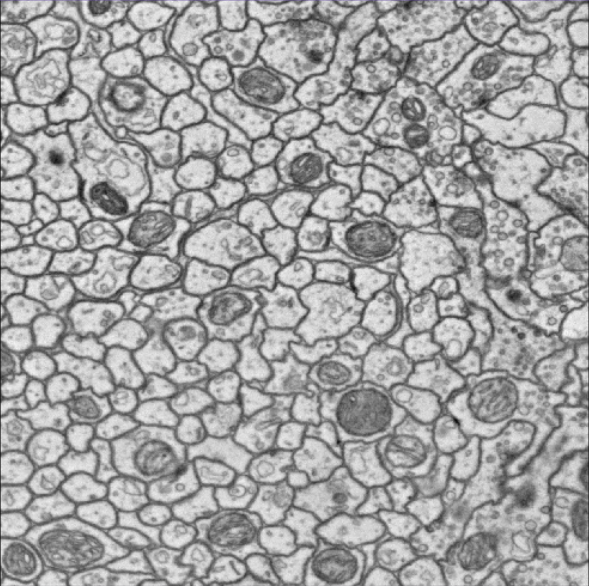
\includegraphics[height=1.2in]{./images/cremi_orig_1.png}
        \caption{Original image}
    \end{subfigure}%
    ~ 
    \begin{subfigure}[t]{0.45\textwidth}
        \centering
        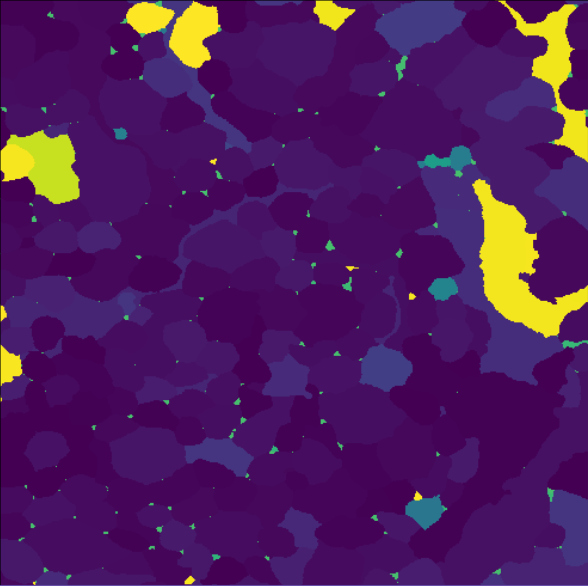
\includegraphics[height=1.2in]{./images/cremi_gt_1.png}
        \caption{Groundtruth}
    \end{subfigure}
    \caption{CREMI dataset (volume A)}
\end{figure}

Our 3D image of size X x Y x Z was easier to predict in two-dimension. 
That's why we considered Z images of size X x Y which were stacked together to get back a 3D image.\\


A question arises : how to get an image segmentation from the affinity graph ?\\

We used two different methods to answer this problem.\\
First of all, a BPT (Binary Partition Tree) and a graph cut could get a good image segmentation. 

\begin{figure}[!htbp]
	\centering
	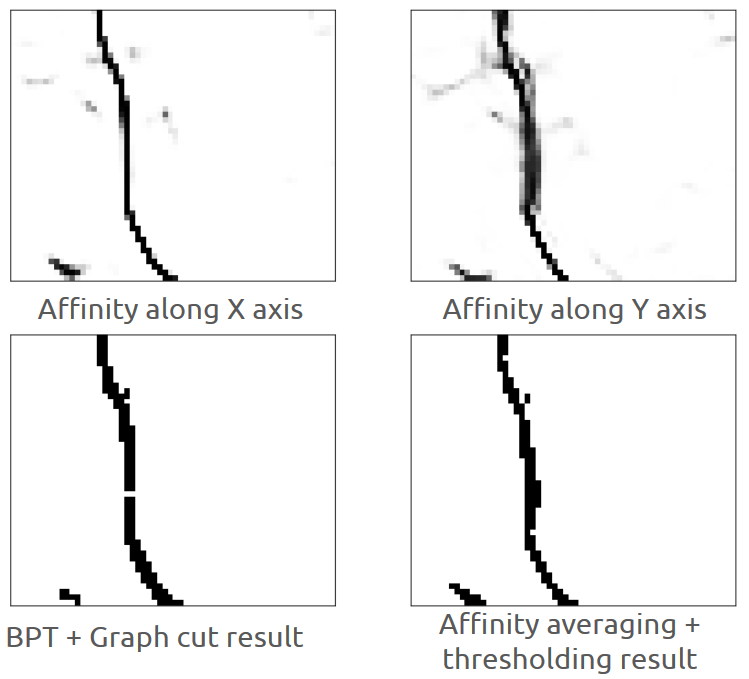
\includegraphics[width=0.8\linewidth]{./images/cremi_isthmus.png}
	\caption{Illustration of the isthmus issue in our segmentation}%
	\label{fig:cremi_isthmus}
\end{figure}

However, even with a strong threshold (around 0.99), isthmus appeared and fusion two different objects together.
It's a big issue as it affects our scores.\\
Secondly, to get rid of isthmus, we did an average affinity and it could segmented the objects nicely.\\
Isthmus issues can be solved by improving our post-processing, and it should disappear with a better architecture.\\

\begin{figure}[!htbp]
    \centering
    \begin{subfigure}[t]{0.31\textwidth}
        \centering
        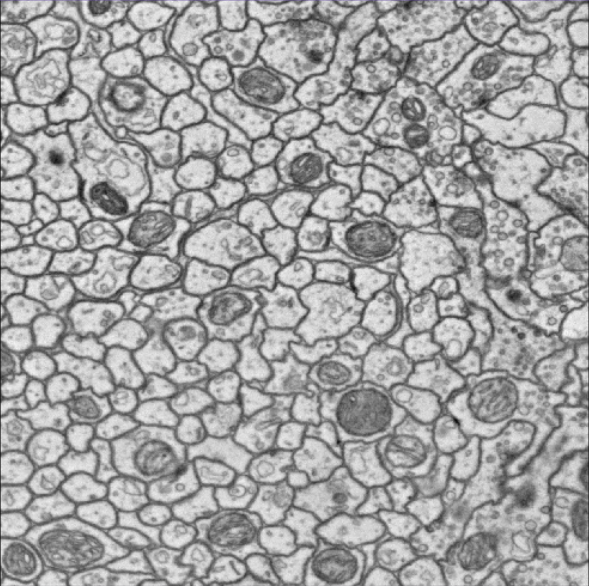
\includegraphics[height=1.2in]{./images/cremi_orig_1.png}
        \caption{Original image}
    \end{subfigure}%
    \begin{subfigure}[t]{0.31\textwidth}
        \centering
        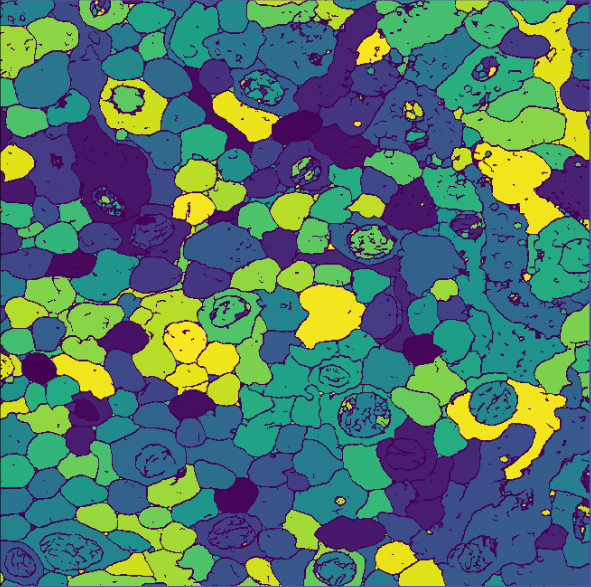
\includegraphics[height=1.2in]{./images/cremi_out_1.png}
        \caption{Our segmentation}
    \end{subfigure}%
    \begin{subfigure}[t]{0.31\textwidth}
        \centering
        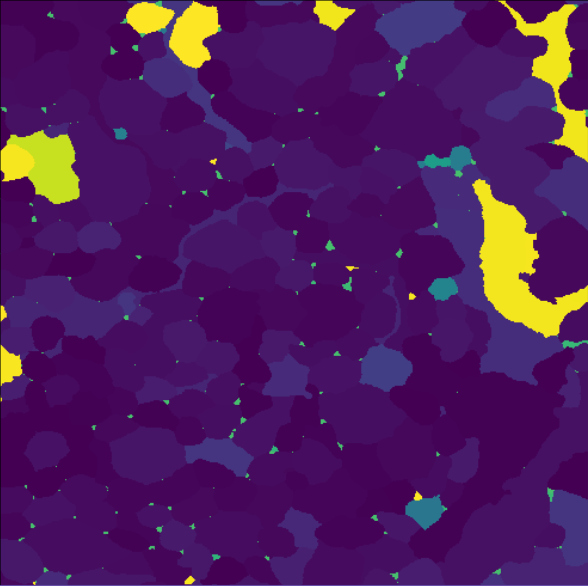
\includegraphics[height=1.2in]{./images/cremi_gt_1.png}
        \caption{Groundtruth}
    \end{subfigure}
    \caption{Results of our training on the CREMI volume A}
\end{figure}

Our results are promising as the different objects are well segmented. 
Yet, there are a few oversegmentations when regions are darker.\\ 
Nucleus are not detected as a same object as the cell.\\

\textcolor{red}{add volume B test}
\begin{figure}[!htbp]
    \centering
    \begin{subfigure}[t]{0.31\textwidth}
        \centering
        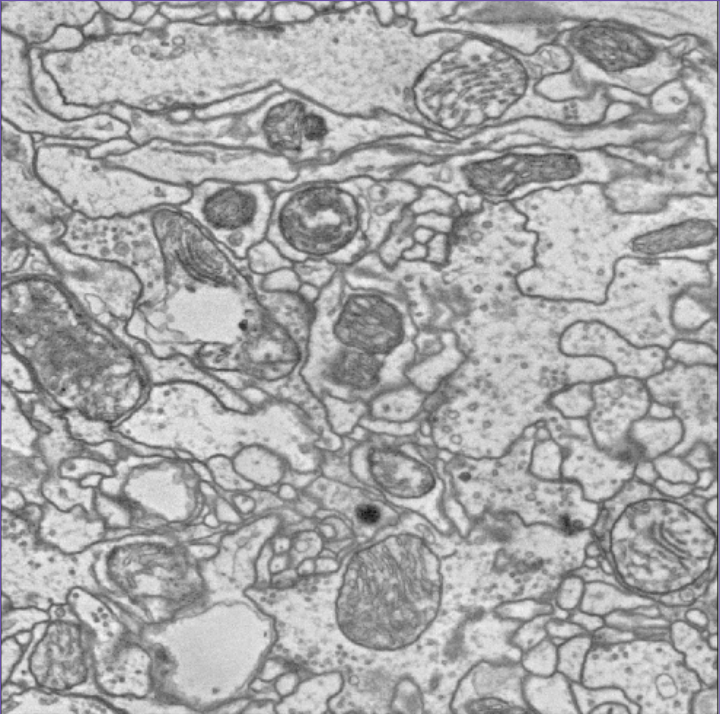
\includegraphics[height=1.2in]{./images/cremi_orig_2.png}
        \caption{Original image}
    \end{subfigure}%
    ~ 
    \begin{subfigure}[t]{0.31\textwidth}
        \centering
        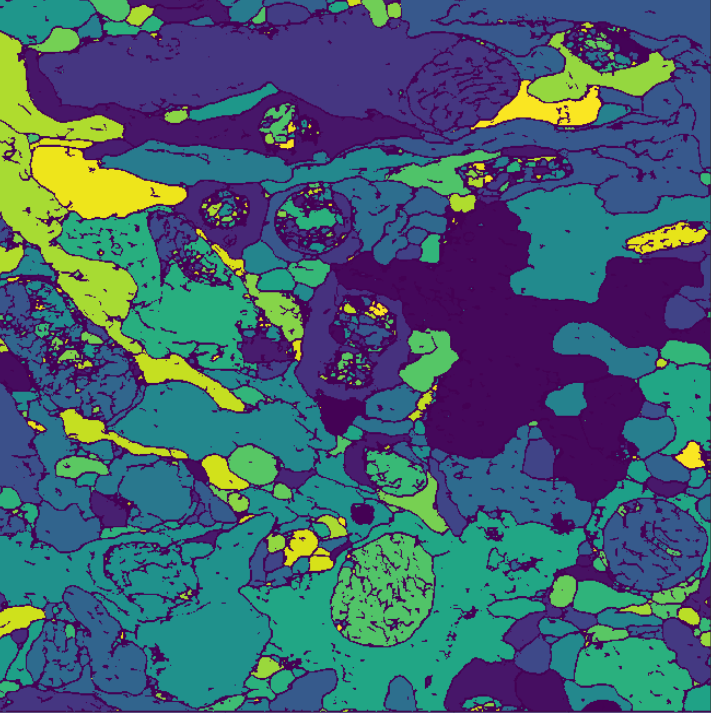
\includegraphics[height=1.2in]{./images/cremi_out_2.png}
        \caption{Our segmentation}
    \end{subfigure}
    ~ 
    \begin{subfigure}[t]{0.31\textwidth}
        \centering
        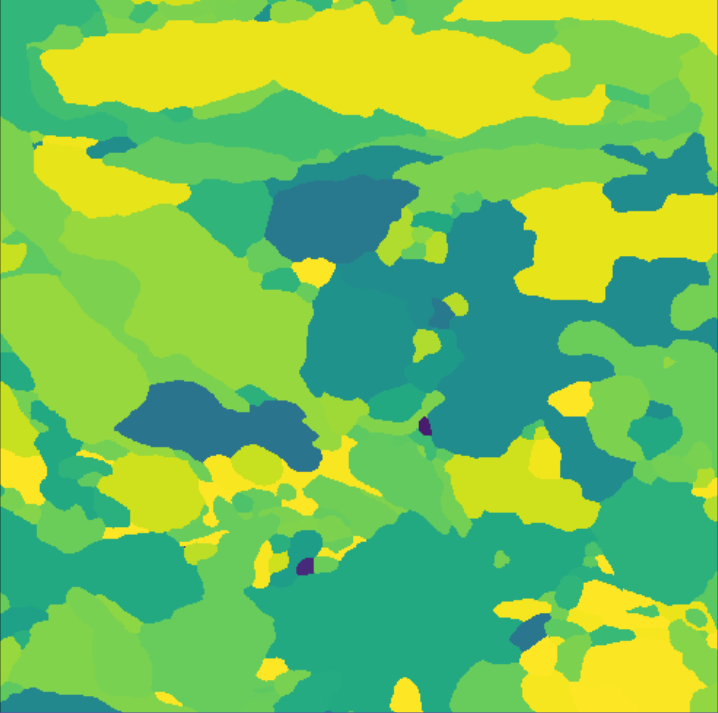
\includegraphics[height=1.2in]{./images/cremi_gt_2.png}
        \caption{Groundtruth}
    \end{subfigure}
    \caption{Results of our test on the CREMI volume B}
\end{figure}

The second volume (volume B) was used as the test set.
The image was similar to the one in the first volume but the objects are more stretched out.\\
Here the objects are well segmented but it was harder on darker regions.\\

With more details, we can evaluate with numerical results, according to the Rand index and the VOI (variation of information) merge and split. 
\textcolor{red}{"The Rand index is a measure of the similarity between two data clustering."
*explain VOI*\\}
The Rand index should be the highest as possible, closer to 1. 
The metric VOI should be lower to be better.\\

\begin{table}[!htbp]
	\centering
	\begin{tabular}{|c|c|c|c|}
		\hline
		& Rand index & \thead{VOI merge \\(lower is better)} & \thead{VOI split\\(lower is better)} \\
		\hline
		\makecell{MALIS : Training set \\(original architecture)} & 0.53 & 2.08 & 1.32\\
		\hline
		MALIS : Training set & 0.61 & 1.25 & 1.03\\
		\hline
		MALIS : Test set & 0.53 & 1.57 & 1.38\\
		\hline
	\end{tabular}
	\caption{Results on the CREMI dataset}
\label{tab:cremi_res}
\end{table}

In the original architecture of 4 layers, the Rand index is 0.53 while we got 0.61 with our training set and 0.53 with our test set.
Our Rand index is higher to the one of the original architecture.
Moreover our VOI is low so it's corresponding to our desired outcome.\\

Thus, our results are hopeful knowing our architecture used was really simple.\\ 
It's still far from the state of the art but it could get even better with a more complex network.\\

\subsection{ISBI 2012}
In a second part, we evaluated our method on the ISBI 2012 Challenge dataset which is a set of 30 sections from a serial section Transmission Electron Microscopy (ssTEM) data set of Drosophila first instar larva ventral nerve cord(VNC).\\

\begin{figure}[!htbp]
    \centering
	\begin{subfigure}[t]{0.31\textwidth}
        \centering
        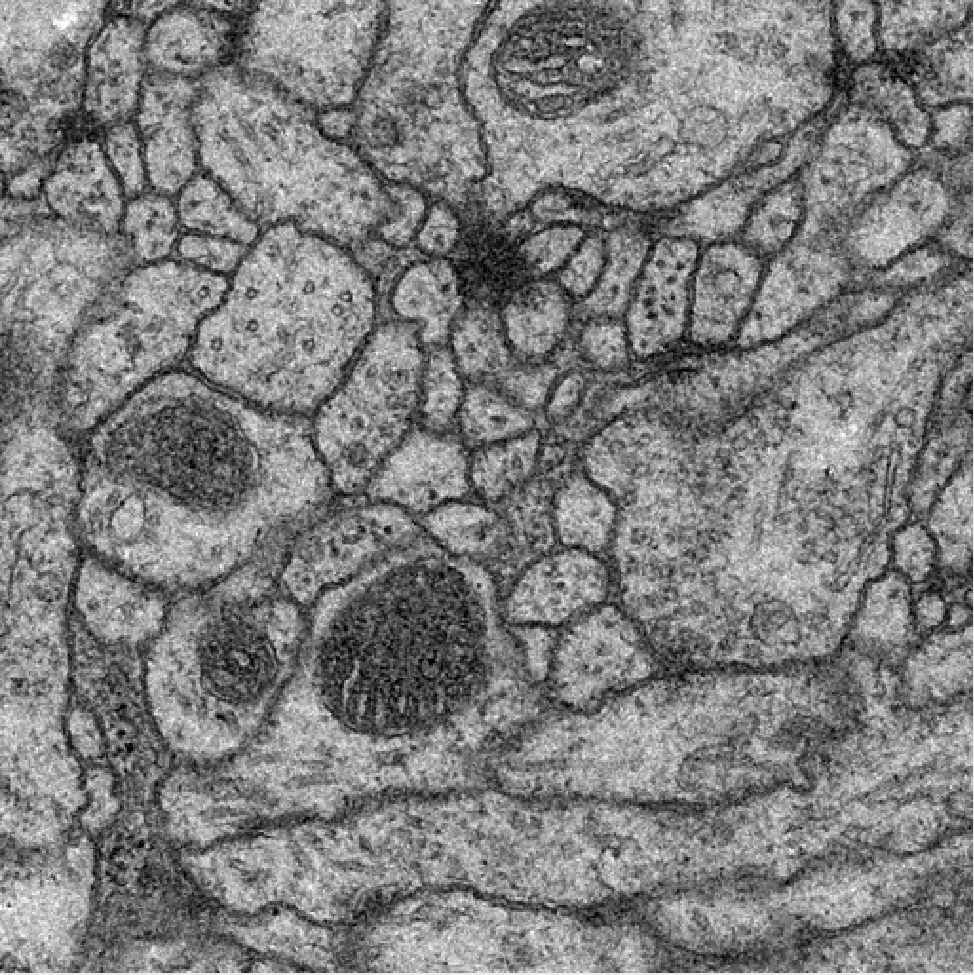
\includegraphics[height=1.2in]{./images/isbi_orig_1.png}
        \caption{Original image}
    \end{subfigure}%
    \begin{subfigure}[t]{0.31\textwidth}
        \centering
        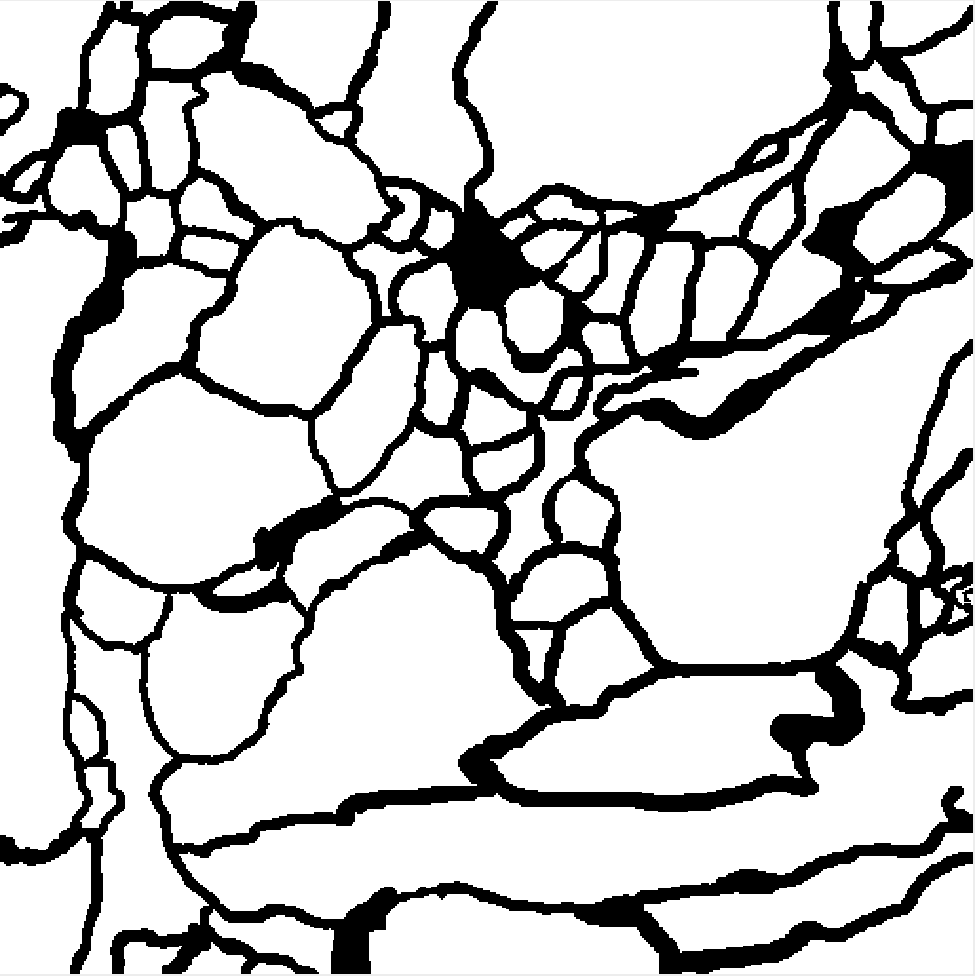
\includegraphics[height=1.2in]{./images/isbi_gt_1.png}
        \caption{Groundtruth}
    \end{subfigure}
    \caption{ISBI dataset example}
\end{figure}

The dataset also provides a corresponding groundtruth with labeled connected components, and thick contours.\\
There is no test set available because we should submit our method to the challenge's leaderboard to get our scores.
The image has a size of 512x512x30 which is smaller than the CREMI's.\\
We evaluated using FIJI (Fiji Is Just Imagej) as an evaluation script was given
for it in the challenge.\\

The same architecture that we used for the CREMI dataset was used for the ISBI dataset.\\

\begin{figure}[!htbp]
    \centering
    \begin{subfigure}[t]{0.31\textwidth}
        \centering
        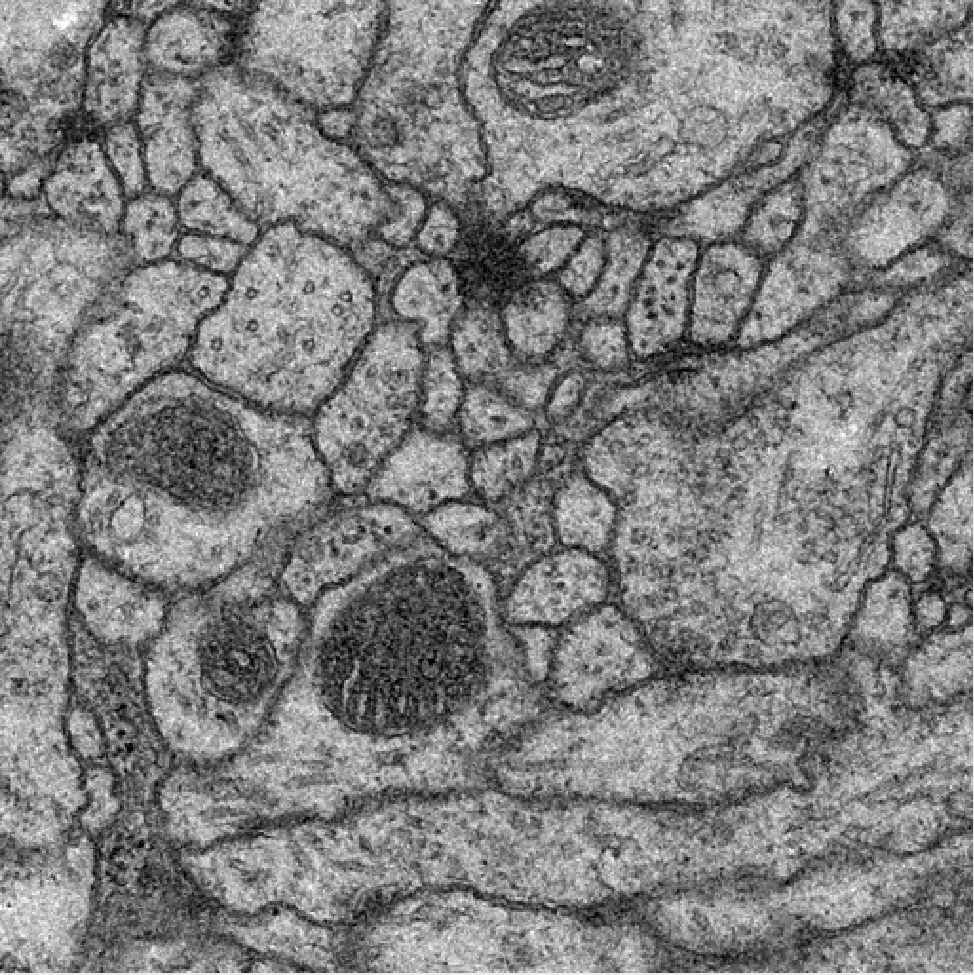
\includegraphics[height=1.2in]{./images/isbi_orig_1.png}
        \caption{Original image}
    \end{subfigure}%
    \begin{subfigure}[t]{0.31\textwidth}
        \centering
        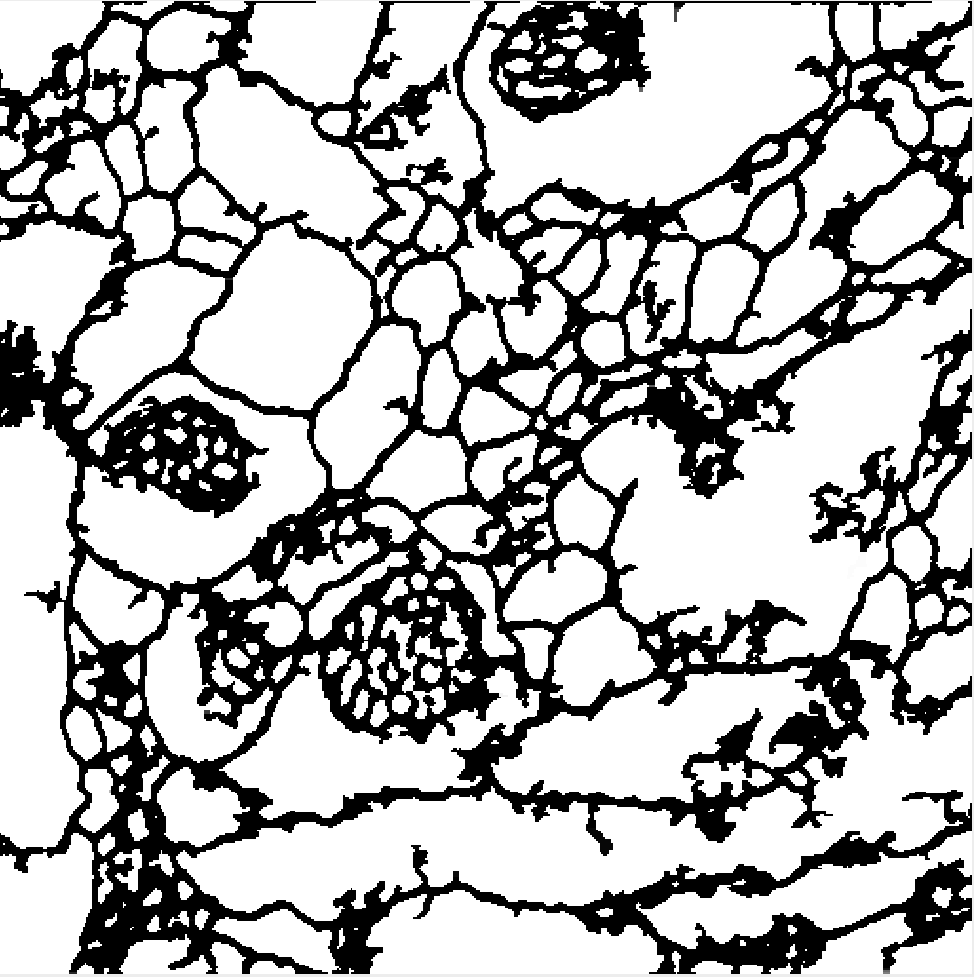
\includegraphics[height=1.2in]{./images/isbi_out_1.png}
        \caption{Our segmentation}
    \end{subfigure}
    \begin{subfigure}[t]{0.31\textwidth}
        \centering
        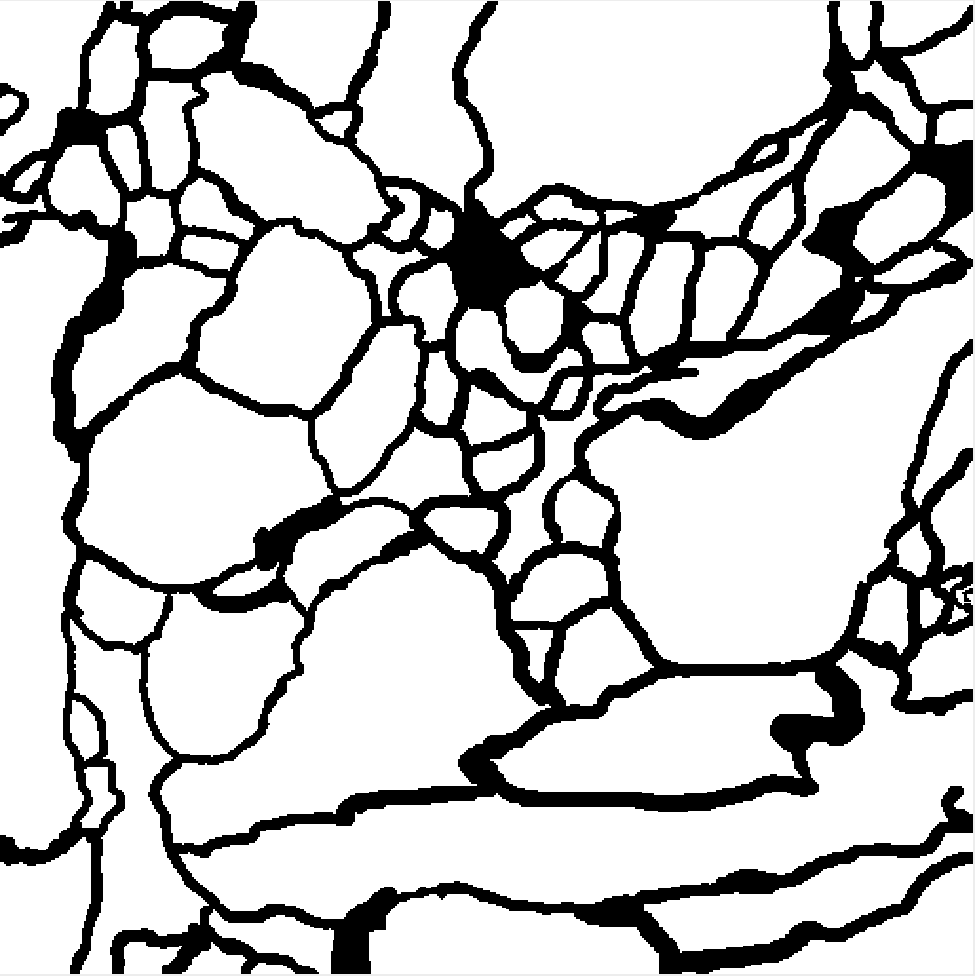
\includegraphics[height=1.2in]{./images/isbi_gt_1.png}
        \caption{Groundtruth}
    \end{subfigure}
    \caption{Results of our training on the ISBI dataset}
\end{figure}

We still get good results even with a simple architecture, because the different objects are well seperated.
However, there are oversegmentations for darker regions as well.

\begin{figure}[!htbp]
    \centering
    \begin{subfigure}[t]{0.31\textwidth}
        \centering
        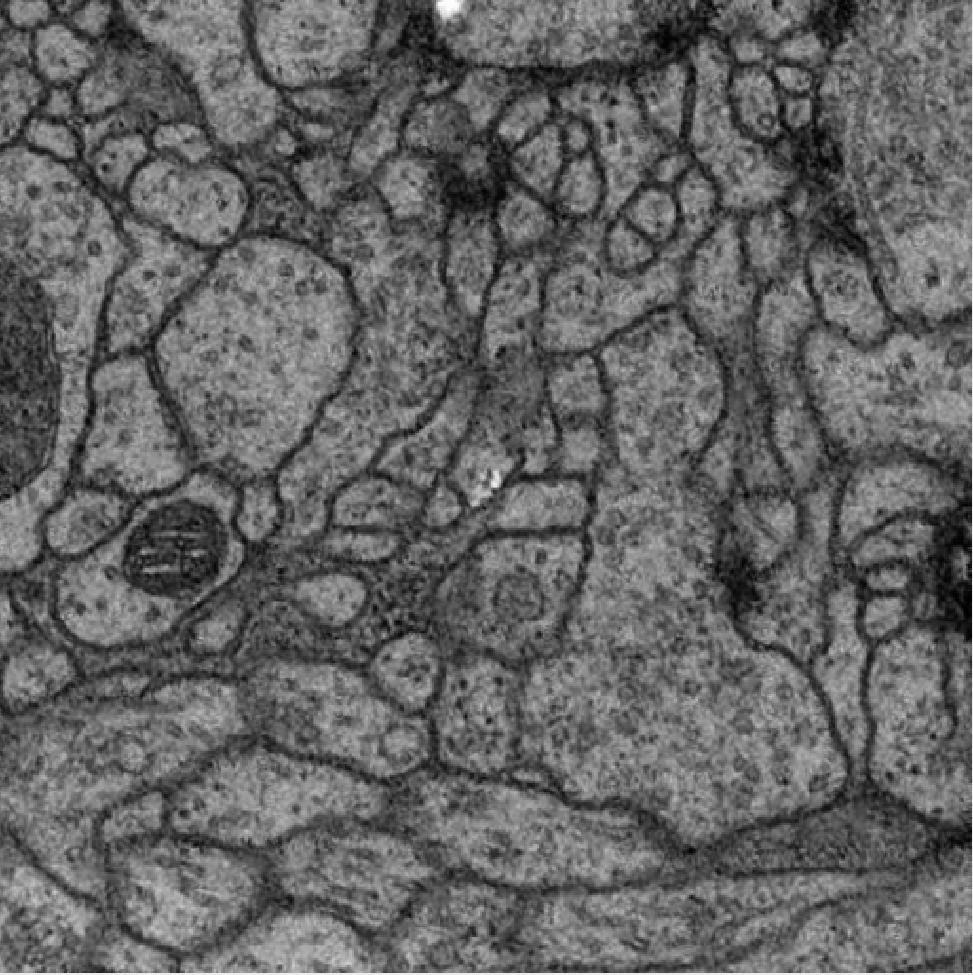
\includegraphics[height=1.2in]{./images/isbi_orig_2.png}
        \caption{Original image}
    \end{subfigure}%
    \begin{subfigure}[t]{0.31\textwidth}
        \centering
        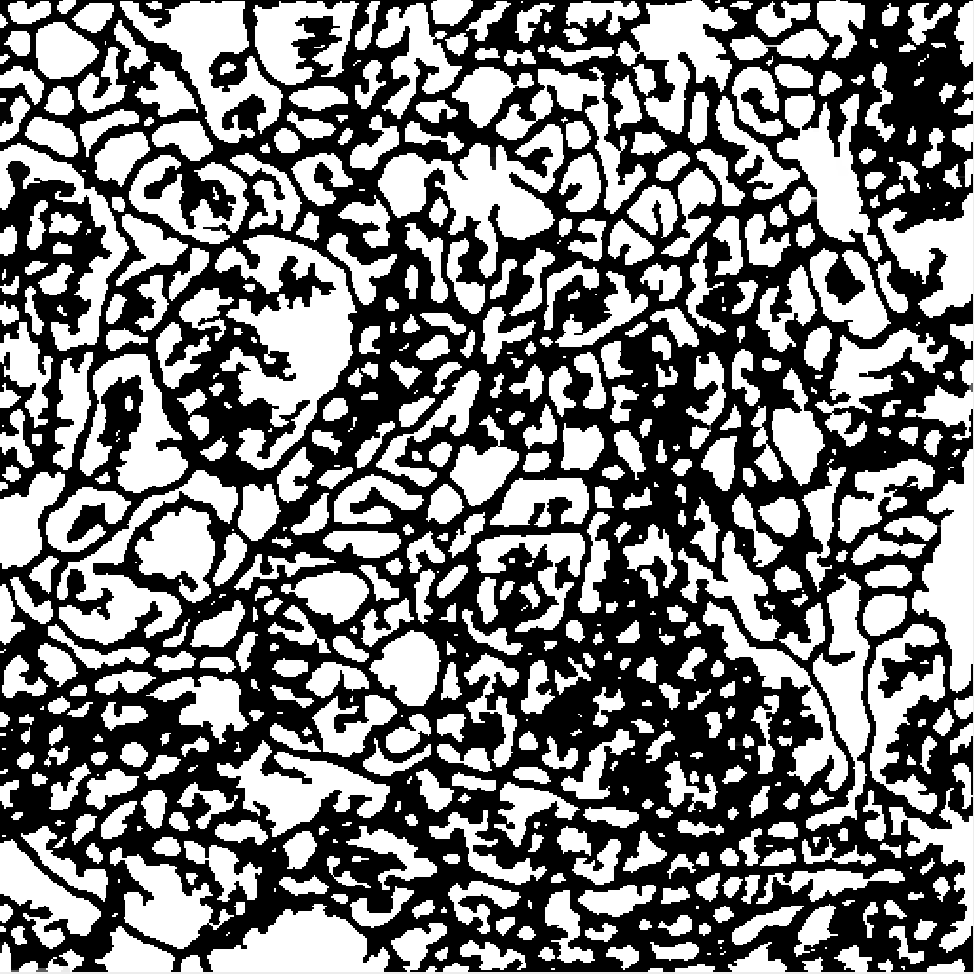
\includegraphics[height=1.2in]{./images/isbi_out_2.png}
        \caption{Our segmentation}
    \end{subfigure}
    \begin{subfigure}[t]{0.31\textwidth}
        \centering
        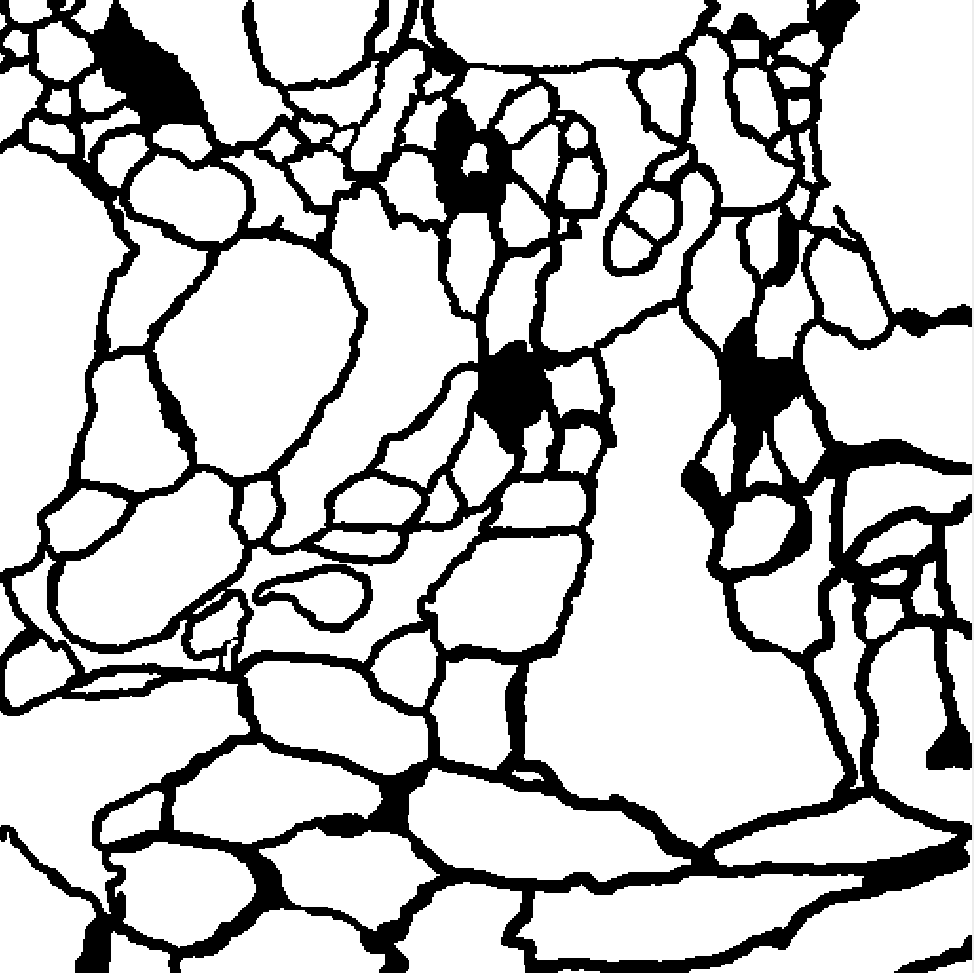
\includegraphics[height=1.2in]{./images/isbi_gt_2.png}
        \caption{Groundtruth}
    \end{subfigure}
    \caption{Results of our test on the ISBI dataset}
\end{figure}

For example, in the figure above, there a lot of oversegmentations. This is one of worst image segmentation among the whole dataset.\\
This image is also the darkest, that's why we made the hypothesis that the oversegmentation issue come from the lack of contrast of the image.\\

To get numerical results we had to submit our method to the ISBI challenge.\\
We evaluate through the same metrics as for the CREMI dataset, that is to say the Rand index and the VOI.
This time the VOI should be higher to be better.\\

\begin{table}[!htbp]
	\centering
	\begin{tabular}{|c|c|c|}
		\hline
		& Rand index & VOI \\
		\hline
		MALIS : Training set & 0.76 & 0.89\\
		\hline
		MALIS : Test set & 0.73 & 0.87\\
		\hline
		Thresholding : Test set & 0.752 & 0.82\\
		\hline
	\end{tabular}
	\caption{Results on the ISBI dataset}
	\label{tab:isbi_res}
\end{table}

The Rand index of our training set was 0.76 and 0.73 for the test test, which is similar but still higher than the thresholding with a Rand index of 0.72.
Our VOI is also a bit higher than the threshold.\\
Those are better results than CREMI's probably due to the small size of the image and the thick borders of the segmentation.\\ 
It means we could have very promising results with our actual method.
We could get even closer to the state of the art if we adopt an improved method.\\


